\chapter{User Testing}

This chapter describes the methodology and results of user testing conducted on the previously proposed and designed gamification features for English Mind. The testing focused on evaluating the clarity, intuitiveness, and potential effectiveness of the new gamification elements.

\section{Testing Methodology}

Two distinct user groups were selected for testing to provide diverse perspectives. Group A consisted of participants with prior experience using language learning applications, while Group B included participants without significant experience in this area.

\begin{itemize}
    \item \textbf{Group A (Experienced Users):}
    \begin{itemize}
        \item 3 participants aged 18-45
        \item Regular users of apps like Duolingo, WordUp, or Duocards
        \item Familiar with gamification concepts through regular usage of language learning applications (even without knowing the formal terminology)
    \end{itemize}

    \item \textbf{Group B (Novice Users):}
    \begin{itemize}
        \item 3 participants aged 18-45
        \item Interest in learning English vocabulary
        \item Limited exposure to language learning applications
    \end{itemize}
\end{itemize}

The testing was conducted in a controlled, quiet environment where participants interacted with high-fidelity interactive prototypes on mobile devices. Each session lasted between 30-45 minutes and was documented through screen and audio recordings.

Data collection during the testing sessions combined several methods to gather comprehensive feedback about the gamification features. Participants were encouraged to think aloud while interacting with the prototype, sharing their thoughts and reactions to different elements. This verbal feedback was supplemented by observation notes documenting user behavior, particularly noting any points of confusion or excitement. After completing the test scenario (see Section \ref{sec:test-scenario}), participants filled out a structured questionnaire rating various aspects of the gamification features on a 5-point Likert scale (see Table \ref{tab:questionnaire}). The questionnaire focused on key metrics such as feature clarity, perceived usefulness, and likelihood of maintaining engagement.


\begin{table}[h]
    \centering
    \caption{User Testing Questionnaire}
    \label{tab:questionnaire}
    \makebox[\textwidth][c]{
        \begin{tabular}{|p{0.9\textwidth}|c|c|c|c|c|}
            \hline
            \multicolumn{6}{|l|}{\small 1 = Strongly Disagree, 2 = Disagree, 3 = Neutral, 4 = Agree, 5 = Strongly Agree} \\
            \hline
            \textbf{Question} & \textbf{1} & \textbf{2} & \textbf{3} & \textbf{4} & \textbf{5} \\
            \hline
            \multicolumn{6}{|l|}{\textbf{Practice Flashcards Experience}} \\
            \hline
            1. The different types of flashcards made practice more engaging & & & & & \\
            \hline
            2. Each flashcard type's instructions were clear and easy to understand & & & & & \\
            \hline
            3. The variety in flashcard types helped me learn vocabulary more effectively & & & & & \\
            \hline
            4. The distribution of different flashcard types felt well-balanced & & & & & \\
            \hline
            5. The five-stage individual word progress indicator was easy to understand & & & & & \\
            \hline
            6. Seeing my progress for individual words motivated me to practice more & & & & & \\
            \hline
            7. The individual word progress indicator's placement was visually clear without being distracting & & & & & \\
            \hline
            8. I found the progress tracking helpful for understanding my learning journey & & & & & \\
            \hline
            9. The practice statistics provided useful information about my session & & & & & \\
            \hline
            10. The celebratory animations made completing practice more rewarding & & & & & \\
            \hline
            11. The review screen motivated me to complete future practice sessions & & & & & \\
            \hline
            \multicolumn{6}{|l|}{\textbf{Streak System}} \\
            \hline
            12. The streak system's requirements were clear and easy to understand & & & & & \\
            \hline
            13. The visual states (active/at risk) effectively communicated streak status & & & & & \\
            \hline
            14. The celebration screen for maintaining streaks felt rewarding & & & & & \\
            \hline
            15. The requirement to learn one new word daily feels achievable & & & & & \\
            \hline
            16. The streak system would help me build a consistent practice habit & & & & & \\
            \hline
            17. I would be more likely to use the app regularly because of the streak feature & & & & & \\
            \hline
            \multicolumn{6}{|l|}{\textbf{Overall Experience}} \\
            \hline
            18. The gamification features enhanced my learning experience & & & & & \\
            \hline
            19. The features felt well-integrated with the app's educational purpose & & & & & \\
            \hline
            20. The gamification elements maintained my interest without being distracting & & & & & \\
            \hline
            21. I would recommend this app to others learning English vocabulary & & & & & \\
            \hline
            22. I would continue using this app for long-term vocabulary learning & & & & & \\
            \hline
        \end{tabular}
    }
\end{table}

\section{Test Scenario}
\label{sec:test-scenario}
The test scenario consists of two main phases: understanding the streak system and completing a practice session. This approach allows evaluation of both the gamification mechanics and their integration into the learning experience:

\begin{enumerate}
    \item \textbf{Phase 1: Streak System}
    \begin{itemize}
        \item Understanding streak activation and maintenance requirements
        \item Interpreting streak status indicators
        \item Initial feedback on motivational aspects
    \end{itemize}
    
    \item \textbf{Phase 2: Practice Flashcards Session}
    \begin{itemize}
        \item {Various Flashcard Types}
        \begin{itemize}
            \item Clarity of instructions for each flashcard type 
            \item Perceived value of variety in maintaining engagement
            \item Comfort level with each flashcard type's interaction method
        \end{itemize}

        \item {Individual Word Progress Tracking}
        \begin{itemize}
            \item Recognition and interpretation of the five-stage progress indicator
            \item Visibility and placement of the progress indicator
            \item Motivational impact of seeing word progress
        \end{itemize}

        \item {Post-Practice Review}
        \begin{itemize}
            \item Comprehension of practice statistics
            \item Impact of celebratory animations and mascot interactions
            \item Understanding of how the completed session affects their streak
        \end{itemize}
    \end{itemize}
\end{enumerate}

The testing process employs a think-aloud protocol, where participants verbalize their thoughts while interacting with the prototype. Initially, participants demonstrate their understanding of the streak system to the interviewer. They then proceed through a complete practice session, experiencing the integrated gamification elements. Throughout both phases, participants provide continuous feedback on interface clarity, emotional engagement, perceived long-term motivation potential, and any usability concerns. This structured approach enables comprehensive evaluation of both immediate user experience and potential sustained engagement with the application.

\newpage

\section{Results and Evaluation}

The user testing results, as detailed in Table \ref{tab:questionnaire-results}, provide valuable insights into the effectiveness and areas for improvement of the gamification features in the English Mind application.

Overall, the feedback was positive, with participants appreciating the variety and engagement offered by the different flashcard types. The overall average rating across all questionnaire items was 4.5, indicating a generally favorable reception of the gamification elements. However, the testing also highlighted several areas needing improvement:

\begin{itemize}
    \item \textbf{"Can't Speak Now" Button Confusion}: Some users were confused by the prominence of the "Can't Speak Now" button, mistaking it for the primary action in the pronunciation flashcard type (see Figure \ref{fig:em-testing-pronunciation-before-after}).
    
    \textit{Solution}: Prioritize the pronunciation button with the microphone icon as the main call-to-action. This can be achieved by enhancing its size, color, or positioning to make it more prominent and intuitive for users.

    \begin{figure}[!h]
        \centering
        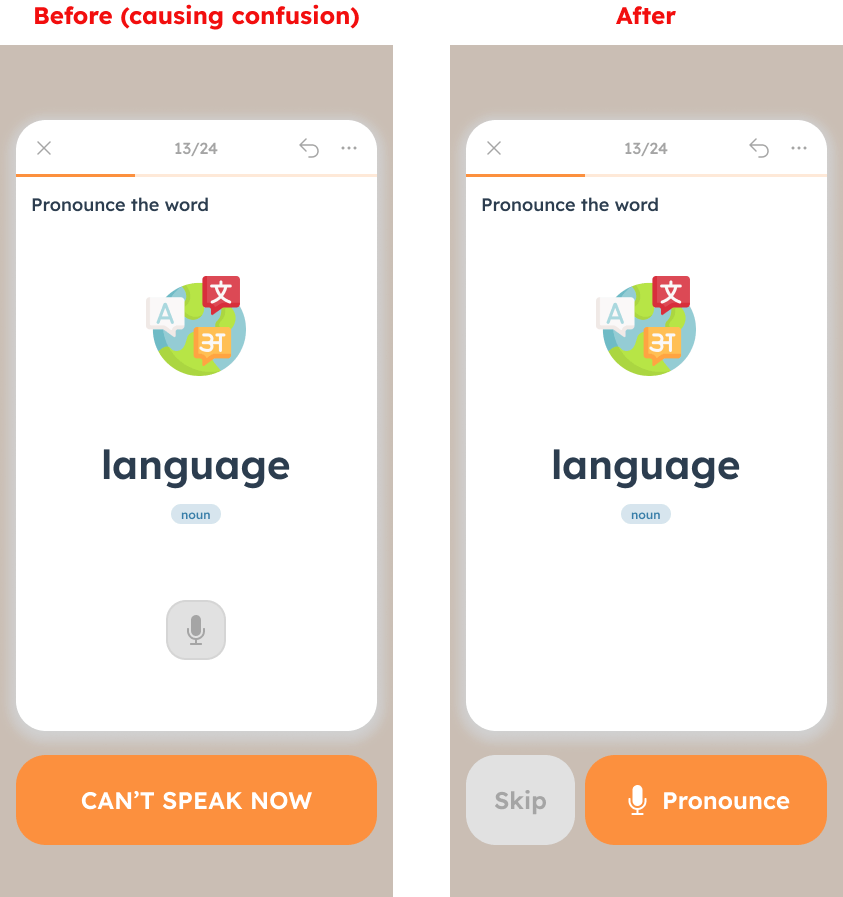
\includegraphics[width=0.75\textwidth]{src/figures/em-testing-pronunciation-before-after.png}
        \caption{Comparison of pronunciation interface before and after improvements}
        \label{fig:em-testing-pronunciation-before-after}
    \end{figure}
    
    \item \textbf{Matching Flashcard Instructions}: Users initially experienced confusion with the matching flashcard type, although they quickly figured it out.
    
    \textit{Solution}: Add brief, clear instructions or visual cues to guide users on how to interact with this flashcard type effectively.
    
    \item \textbf{Simplification of Explanations}: The explanation of the word progress indicator was perceived as too detailed and tiring by some participants.
    
    \textit{Solution}: Simplify the explanation by using concise language and visual aids, such as icons or diagrams, to improve user comprehension and reduce cognitive load.
\end{itemize}

These areas of improvement were subsequently adjusted and retested, confirming that the changes enhanced user experience and addressed the initial concerns effectively.

\begin{table}[ht]
    \centering
    \caption{Results of User Testing Questionnaire}
    \label{tab:questionnaire-results}
    \makebox[\textwidth][c]{
        \begin{tabular}{|p{0.76\textwidth}|c|c|c|c|c|c|c|}
            \hline
            \multicolumn{8}{|l|}{\small A1, A2, A3 = Experienced Users; B1, B2, B3 = Novice Users; Avg = Average} \\
            \multicolumn{8}{|l|}{\small 1 = Strongly Disagree, 2 = Disagree, 3 = Neutral, 4 = Agree, 5 = Strongly Agree} \\
            \hline
            \textbf{Question} & \textbf{A1} & \textbf{A2} & \textbf{A3} & \textbf{B1} & \textbf{B2} & \textbf{B3} & \textbf{Avg} \\
            \hline
            \multicolumn{8}{|l|}{\textbf{Practice Flashcards Experience}} \\
            \hline
            1. The different types of flashcards made practice more engaging & 5 & 5 & 5 & 5 & 5 & 5 & 5.0 \\
            \hline
            2. Each flashcard type's instructions were clear and easy to understand & 5 & 5 & 4 & 4 & 4 & 4 & 4.3 \\
            \hline
            3. The variety in flashcard types helped me learn vocabulary more effectively & 4 & 4 & 5 & 5 & 4 & 4 & 4.3 \\
            \hline
            4. The distribution of different flashcard types felt well-balanced & 4 & 5 & 4 & 5 & 5 & 5 & 4.7 \\
            \hline
            5. The five-stage individual word progress indicator was easy to understand & 5 & 5 & 3 & 4 & 4 & 3 & 4.0 \\
            \hline
            6. Seeing my progress for individual words motivated me to practice more & 4 & 3 & 3 & 4 & 3 & 3 & 3.3 \\
            \hline
            7. The individual word progress indicator's placement was visually clear without being distracting & 2 & 4 & 5 & 5 & 3 & 5 & 4.0 \\
            \hline
            8. I found the progress tracking helpful for understanding my learning journey & 5 & 4 & 5 & 5 & 5 & 4 & 4.7 \\
            \hline
            9. The practice statistics provided useful information about my session & 5 & 4 & 5 & 5 & 4 & 5 & 4.7 \\
            \hline
            10. The celebratory animations made completing practice more rewarding & 5 & 4 & 5 & 5 & 4 & 5 & 4.7 \\
            \hline
            11. The review screen motivated me to complete future practice sessions & 5 & 5 & 5 & 4 & 3 & 5 & 4.5 \\
            \hline
            \multicolumn{8}{|l|}{\textbf{Streak System}} \\
            \hline
            12. The streak system's requirements were clear and easy to understand & 5 & 5 & 4 & 5 & 4 & 5 & 4.7 \\
            \hline
            13. The visual states (active/at risk) effectively communicated streak status & 5 & 5 & 3 & 5 & 4 & 4 & 4.3 \\
            \hline
            14. The celebration screen for maintaining streaks felt rewarding & 5 & 4 & 5 & 5 & 4 & 5 & 4.7 \\
            \hline
            15. The requirement to learn one new word daily feels achievable & 5 & 5 & 5 & 5 & 5 & 5 & 5.0 \\
            \hline
            16. The streak system would help me build a consistent practice habit & 5 & 4 & 5 & 4 & 4 & 5 & 4.5 \\
            \hline
            17. I would be more likely to use the app regularly because of the streak feature & 5 & 5 & 4 & 3 & 4 & 4 & 4.2 \\
            \hline
            \multicolumn{8}{|l|}{\textbf{Overall Experience}} \\
            \hline
            18. The gamification features enhanced my learning experience & 5 & 4 & 5 & 4 & 5 & 5 & 4.7 \\
            \hline
            19. The features felt well-integrated with the app's educational purpose & 4 & 5 & 5 & 5 & 5 & 5 & 4.8 \\
            \hline
            20. The gamification elements maintained my interest without being distracting & 4 & 5 & 5 & 5 & 5 & 5 & 4.8 \\
            \hline
            21. I would recommend this app to others learning English vocabulary & 5 & 5 & 5 & 5 & 5 & 5 & 5.0 \\
            \hline
            22. I would continue using this app for long-term vocabulary learning & 5 & 4 & 5 & 4 & 4 & 5 & 4.5 \\
            \hline
        \end{tabular}
    }
\end{table}